\section{Ejercicio 1}
\lstinputlisting[language={[Motorola68k]Assembler}]{code/ej1.asm} 

Tomando los registros con los siguientes valores iniciales:

$$ a = \$ffffffffffffff $$
$$ b = \$ffffffffffffff $$
$$ x = \$ffffffffffff $$

% Please add the following required packages to your document preamble:
% \usepackage{multirow}
\begin{table}[H]
\centering
\begin{tabular}{|c|c|c|}
\hline
Instruccion                     & Cambios                               & Comentarios                                        \\ \hline
                                & a = \$ffffffffffffff                  &                                                    \\
-                               & b = \$ffffffffffffff                  & Carga inicial de valores                           \\
                                & x = \$ffffffffffff                    &                                                    \\ \hline
\multirow{3}{*}{move \#\$3d,x1} & \multirow{3}{*}{x = \$3d0000ffffff}   & Se carga el valor de 8 bit interpretado            \\
                                &                                       & como un número signado fraccionario,               \\
                                &                                       & por lo cual se alinea a la izquierda.              \\ \hline
\multirow{3}{*}{move \#\$3d,a1} & \multirow{3}{*}{a = \$ff00003dffffff} & Se carga el valor \$3d solo en el registro $a\_1$  \\
                                &                                       & interpretado como entero no signado                \\
                                &                                       & sin modificar $a_2$ y $a_0$                        \\ \hline
\multirow{4}{*}{move \#\$3d,b}  & \multirow{4}{*}{b = \$003d00000000}   & Se guarda el valor \$3d en el acumulador b         \\
                                &                                       & interpretandolo como numero de punto fijo,         \\
                                &                                       & por lo cual se extiende el signo siendo $b_2$ \$00 \\
                                &                                       & y se completa $b_0$ = \$000000\$                  \\ \hline
\end{tabular}
\end{table}


En la tabla~\ref{tab:ej1_results} se muestra el estado final de los registros.

\begin{table}[H]
\centering
\begin{tabular}{|c|c|c|}
\hline
\textbf{Registro} & \textbf{Valor inicial} & \textbf{Valor final}  \\ \hline
a                 & \$ffffffffffffff       & \$ff00003dffffff      \\ \hline
b                 & \$ffffffffffffff       & \$003d0000000000      \\ \hline
x                 & \$ffffffffffff         & \$3d0000ffffff        \\ \hline
\end{tabular}
\caption{Estado inicial y final de los registros.}
\label{tab:ej1_results}
\end{table}

Se adjunta el estado final de los registros simulados.

\begin{figure}[H]
    \centering
    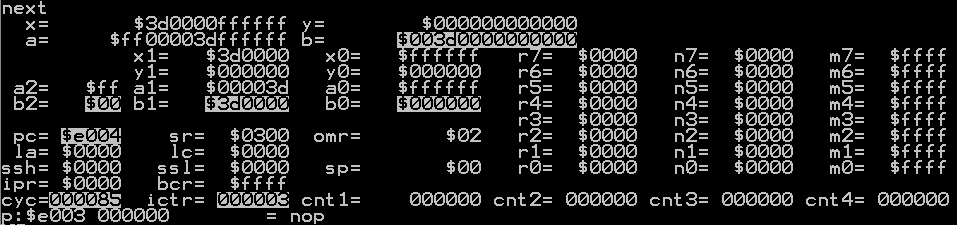
\includegraphics[width=\textwidth]{figs/ej1/3ra_i.png}
    \caption{Estado final de los registros (simulación).}
    \label{fig:ej1_simregs}
\end{figure}
